%\newpage
\section{Forward and Backward Computation}

In Section~\ref{sec:perceptron}, we have explained that a multi-layer perceptron has more expressive power than a single-layer perceptron. In particular, it is able to find a two-layer perceptron to solve the XOR problem, while it is not possible for a single-layer perceptron. However, we did not explain in  Section~\ref{sec:perceptron} how to compute the weights for the two-layer perceptron for XOR. Moreover, we note that, the perceptron learning algorithm cannot be used for learning multi-layer perceptron. Actually, the learning algorithm for multi-layer perceptron, called backpropagation (BP), is one of the key milestones for the development of deep learning. 

The BP algorithm computes the gradient of the loss function with respect to each weight by the chain rule. Instead of computing one gradient for each weight, it is able to compute
the gradient for one layer at a time, and more importantly, it is able to iterate backwards from the last layer to avoid redundant calculations of intermediate terms in the chain rule. This makes it efficient enough to train large scale neural networks. 

The BP algorithm is the foundation of deep learning, and in this section, we use a running example to explain its computation. 

\subsection*{Running Example}

In this example, we have three layers, one input layer, one hidden layer, and one output layer. Each layer has two neurons. The connections between neurons are given in the left diagram of Figure~\ref{fig:network}. 

\begin{figure}[!htbp]
    \centering
    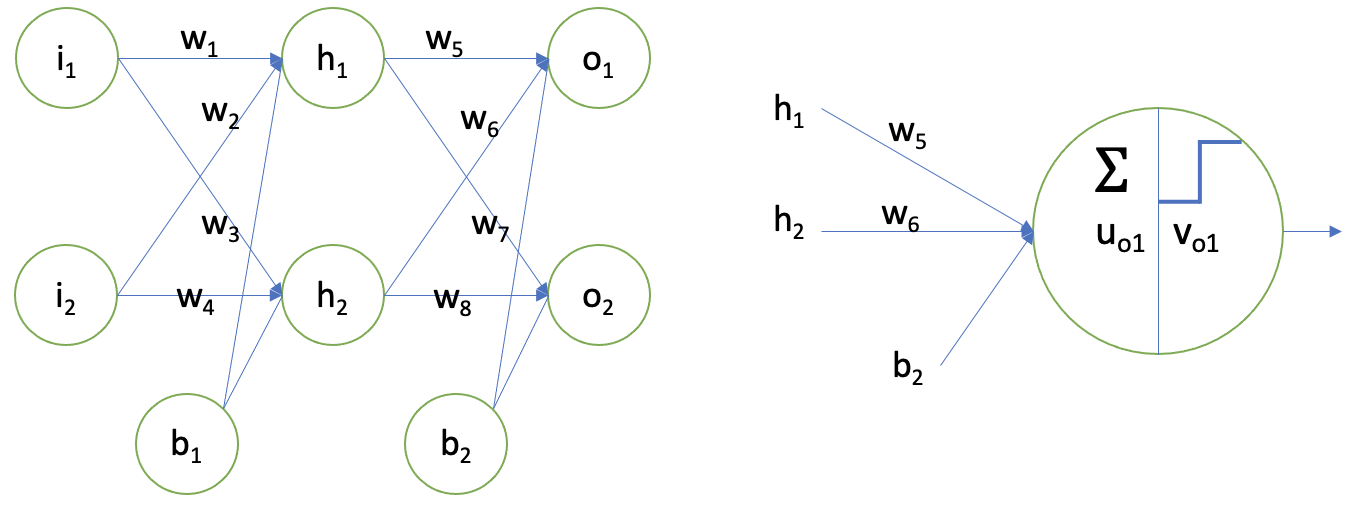
\includegraphics[width=0.8\textwidth]{images/deepLearning/propagation/network.png}
    \caption{A simple neural network with a hidden layer (Left) and the illustration of a neuron with activation function (Right)}
    \label{fig:network}
\end{figure}

The diagram on the right is an illustration of a neuron with an activation function. Each neuron has two values $u$ and $v$, representing its values before and after the application of the activation function, respectively. 

The learning is a dynamic process with weights continuously updated until convergence. Now,  we assume that, at some point, the current weights are 
\begin{equation}
\begin{blockarray}{cc}
\begin{block}{(cc)}
   w_1 & w_2 \\
   w_3 & w_4 \\
\end{block}
\end{blockarray} = 
\begin{blockarray}{cc}
\begin{block}{(cc)}
   0.15 & 0.20 \\
   0.25 & 0.30 \\
\end{block}
\end{blockarray}\text{~~ , ~~}
\begin{blockarray}{cc}
\begin{block}{(cc)}
   w_5 & w_6 \\
   w_7 & w_8 \\
\end{block}
\end{blockarray} = 
\begin{blockarray}{cc}
\begin{block}{(cc)}
   0.40 & 0.45 \\
   0.50 & 0.55 \\
\end{block}
\end{blockarray}
\text{~~ , ~~}
\begin{blockarray}{c}
\begin{block}{(c)}
   b_1 \\
   b_2 \\
\end{block}
\end{blockarray} = 
\begin{blockarray}{c}
\begin{block}{(c)}
   0.35 \\
   0.60 \\
\end{block}
\end{blockarray}
\end{equation}

Note that, every row in a weight matrix stores the input weights for a neuron, for example, the row $(0.15~~0.20)$ is associated with the neuron $h_1$. Also, each entry in a bias vector represents a bias for a layer. 


\subsection{Forward Computation}

The first step of each iteration of the BP algorithm is to compute the loss by making a forward computation. 
%
Assume that we have an input $\textbf{x}=(0.05,0.10)^T$ for the network in Figure~\ref{fig:network}, we can have  

\begin{equation}
\begin{blockarray}{c}
\begin{block}{(c)}
   u_{h_1} \\
   u_{h_2} \\
\end{block}
\end{blockarray} = 
\begin{blockarray}{cc}
\begin{block}{(cc)}
   0.15 & 0.20 \\
   0.25 & 0.30 \\
\end{block}
\end{blockarray} \times 
\begin{blockarray}{c}
\begin{block}{(c)}
   0.05 \\
   0.10 \\
\end{block}
\end{blockarray} +  
\begin{blockarray}{c}
\begin{block}{(c)}
   0.35 \\
   0.35 \\
\end{block}
\end{blockarray} =
\begin{blockarray}{c}
\begin{block}{(c)}
   0.3775 \\
   0.6425 \\
\end{block}
\end{blockarray}
\end{equation}
Assume that the network uses the Sigmoid function $\sigma$ as the activation function, we have 
\begin{equation}
    \begin{blockarray}{c}
\begin{block}{(c)}
   v_{h_1} \\
   v_{h_2} \\
\end{block}
\end{blockarray} = \sigma(
    \begin{blockarray}{c}
\begin{block}{(c)}
   0.3775 \\
   0.3925 \\
\end{block}
\end{blockarray}) \approx 
\begin{blockarray}{c}
\begin{block}{(c)}
   0.5927 \\
   0.5969 \\
\end{block}
\end{blockarray}
\end{equation}
as the output of the hidden layer. 
%
On the output layer, we have 
\begin{equation}
\begin{blockarray}{c}
\begin{block}{(c)}
   u_{o_1} \\
   u_{o_2} \\
\end{block}
\end{blockarray} = 
\begin{blockarray}{cc}
\begin{block}{(cc)}
   0.40 & 0.45 \\
   0.50 & 0.55 \\
\end{block}
\end{blockarray} \times 
\begin{blockarray}{c}
\begin{block}{(c)}
   0.5927 \\
   0.5969 \\
\end{block}
\end{blockarray} +  
\begin{blockarray}{c}
\begin{block}{(c)}
   0.60 \\
   0.60 \\
\end{block}
\end{blockarray} =
\begin{blockarray}{c}
\begin{block}{(c)}
   1.1057 \\
   1.2247 \\
\end{block}
\end{blockarray}
\end{equation}
Consider the Sigmoid function, we have 
\begin{equation}
\begin{blockarray}{c}
\begin{block}{(c)}
   v_{o_1} \\
   v_{o_2} \\
\end{block}
\end{blockarray} =
    \sigma(
    \begin{blockarray}{c}
\begin{block}{(c)}
   1.1057 \\
   1.2247 \\
\end{block}
\end{blockarray}) \approx 
\begin{blockarray}{c}
\begin{block}{(c)}
   0.7513 \\
   0.7729 \\
\end{block}
\end{blockarray}
\end{equation}
as the output of the output layer. That is, $\hat y=(0.7513,0.7729)$. 
%
Now, assuming that the label of $\textbf{x}$ is $y=(0.01,0.99)^T$ and we are using the mean square error, we can compute the loss for 
\begin{equation}
    L(\textbf{x},y) = \frac{1}{2}(0.7513-0.01)^2 + \frac{1}{2}(0.7729-0.99)^2 \approx 0.2748 +0.0236= 0.2984
\end{equation}
where we let $L_{o1}(\textbf{x},y)=\frac{1}{2}(0.7513-0.01)^2$ and $L_{o2}(\textbf{x},y)=\frac{1}{2}(0.7729-0.99)^2$, representing the loss of individual neurons $o_1$ and $o_2$, respectively. 

\subsection{Backward Computation}


Once we have the loss ${L}(\textbf{x},y)$, we can start back-propagation by applying the chain rule. 
%

\subsection*{Weights of output neurons}

First of all, for the weights of output neuron, such as $w_5$, we can compute as follows: 

\begin{equation}\label{equ:backpropoutput}
    \frac{{\partial L}}{{\partial w_5}} = \frac{{\partial L_{o_1}}}{{\partial v_{o_1}}}*\frac{{\partial v_{o_1}}}{{\partial u_{o_1}}}*\frac{{\partial u_{o_1}}}{{\partial w_5}}
\end{equation}
Figure~\ref{fig:backoutput} presents an  illustrative diagram for the Equation (\ref{equ:backpropoutput}). 
\begin{figure}[!htbp]
    \centering
    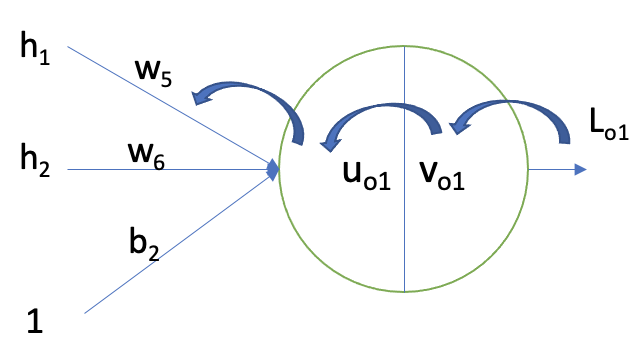
\includegraphics[width=0.4\textwidth]{images/deepLearning/propagation/back.png}
    \caption{Backward propagation on the output neuron}
    \label{fig:backoutput}
\end{figure}
Actually, the backpropagation goes from the loss $L_{o_1}$ to the value $v_{o_1}$, $u_{o_1}$, until the weight $w_5$. 

Concretely, for the running example, we have 
\begin{equation}
     \displaystyle\frac{{\partial L_{o_1}}}{{\partial v_{o_1}}}=\frac{{\partial }}{{\partial v_{o_1}}}(\frac{1}{2}(y^{(1)}-v_{o_1})^2) = -(y^{(1)}-v_{o_1}) = 0.7513-0.01 = 0.74  \\
\end{equation}
where $y^{(1)}$ is the first component of $y$, and 
\begin{equation}
\frac{{\partial v_{o_1}}}{{\partial u_{o_1}}} =  \frac{{\partial \sigma(u_{o_1})}}{{\partial u_{o_1}}} = \sigma(u_{o_1})(1-\sigma(u_{o_1})) = v_{o_1}(1-v_{o_1}) \approx 0.7513\times 0.2487\approx 0.1868
\end{equation}
and 
\begin{equation}
    \frac{{\partial u_{o_1}}}{{\partial w_5}}=\frac{{\partial }}{{\partial w_5}}(w_5v_{h_1}+w_6v_{h_2}+b_2)= v_{h_1} \approx 0.5927
\end{equation}
Therefore, we have 
\begin{equation}
    \frac{{\partial L}}{{\partial w_5}} = \frac{{\partial L_{o_1}}}{{\partial v_{o_1}}}*\frac{{\partial v_{o_1}}}{{\partial u_{o_1}}}*\frac{{\partial u_{o_1}}}{{\partial w_5}}\approx 0.74 \times 0.1868 \times  0.5927 = 0.0819
\end{equation}

\subsection*{Weights of hidden neurons}

Now, the weight of hidden layer can be done recursively by applying the chain rules, e.g., 
\begin{equation}\label{equ:backprophidden}
\begin{array}{rcl}
   \displaystyle  \frac{{\partial L}}{{\partial w_1}} 
   &  = & \displaystyle \frac{{\partial L}}{{\partial v_{h_1}}}*\frac{{\partial v_{h_1}}}{{\partial u_{h_1}}}*\frac{{\partial u_{h_1}}}{{\partial w_1}} \\ 
    & = & \displaystyle (\frac{{\partial L_{o_1}}}{{\partial v_{h_1}}}+\frac{{\partial L_{o_2}}}{{\partial v_{h_1}}})*\frac{{\partial v_{h_1}}}{{\partial u_{h_1}}}*\frac{{\partial u_{h_1}}}{{\partial w_1}} \\
    & = & \displaystyle (\frac{{\partial L_{o_1}}}{{\partial u_{o_1}}}\frac{{\partial u_{o_1}}}{{\partial u_{h_1}}}+\frac{{\partial L_{o_2}}}{{\partial u_{o_2}}}\frac{{\partial u_{o_2}}}{{\partial u_{h_1}}})*\frac{{\partial v_{h_1}}}{{\partial u_{h_1}}}*\frac{{\partial u_{h_1}}}{{\partial w_1}}\\
    & = & \displaystyle (\frac{{\partial L_{o_1}}}{{\partial u_{o_1}}}w_5+\frac{{\partial L_{o_2}}}{{\partial u_{o_2}}}w_7)*\frac{{\partial v_{h_1}}}{{\partial u_{h_1}}}*\frac{{\partial u_{h_1}}}{{\partial w_1}}
\end{array}
\end{equation}
Note that, all the components of Equation (\ref{equ:backprophidden}) can now be computed as the method we used for the output layer. Figure~\ref{fig:backhidden} presents an illustration of backward propagation as in Equation (\ref{equ:backprophidden}). 

\begin{figure}[!htbp]
    \centering
    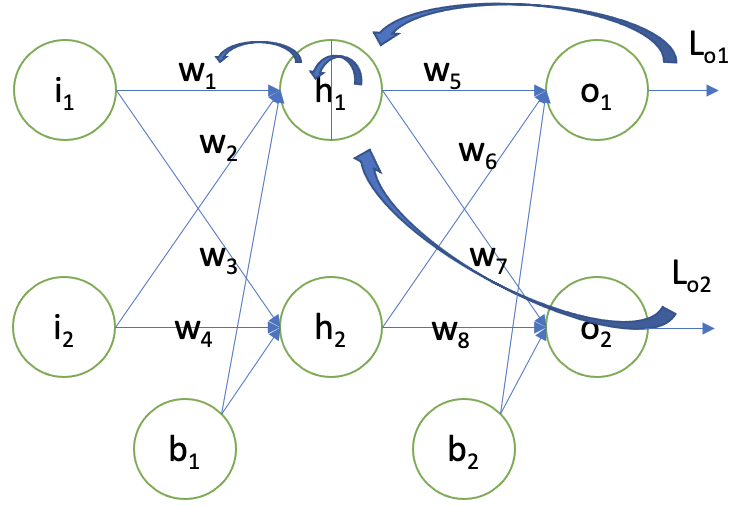
\includegraphics[width=0.45\textwidth]{images/deepLearning/propagation/back2.png}
    \caption{Backward propagation on the hidden neuron}
    \label{fig:backhidden}
\end{figure}

\subsection*{Weight update}

Finally, once we compute the gradients $\displaystyle  \frac{{\partial L}}{{\partial w_5}}$ or $\displaystyle  \frac{{\partial L}}{{\partial w_1}}$, we can update the weights $w_5$ or $w_1$ by applying the gradient descent algorithm. We remark that, while the above computation is conducted for individual weights, the BP algorithm can work on a layer basis to significantly improve the efficiency. 

\subsection{Regularisation as Constraints}

In general, regularisation is a set of methods to  prevent overfitting or help the optimization. Typically, this is done by having additional terms in the training optimisation objective. 

\subsection*{Overfitting}

Overfitting is a concept closely related to the generalisation error as introduced in Section~\ref{sec:generalisationerror}, which is the gap between empirical loss and expected loss. 
It has been observed that, the following two reasons may contribute as the key to the overfitting. 

\begin{itemize}
    \item dataset is too small
    \item hypothesis space is too large
\end{itemize}

To understand the second point, we note that, the larger the hypothesis space, the easier is for a learning algorithm to find a hypothesis that has small training error. However, finding a small training error does not warrant the found hypothesis can be of a small test error, and so this may lead to large test error (overfitting). This observation suggests that it might be beneficial to leave out useless hypotheses, which is what regularization is for. 

\subsection*{Regularization as hard constraint}

Assume that, for a dataset $D=(\textbf{X},\textbf{y})$ of $n$ training instances, we have the following optimising objective: 
\begin{equation}
\begin{array}{rl}
    \displaystyle\min_f & \displaystyle L(f,D) = \frac{1}{n} \sum_{i=1}^n L(f,\textbf{x}_i,y_i) \\
    \text{subject to } & f\in {\cal H}
\end{array}
\end{equation}
Considering that for a deep learning model, $f$ is parameterised over the weights $W$, we have 
\begin{equation}
\begin{array}{rl}
    \displaystyle\min_W & \displaystyle L(W,D) = \frac{1}{n} \sum_{i=1}^n L(W,\textbf{x}_i,y_i) \\
    \text{subject to } & W\in {\cal \real^{|W|}}
\end{array}
\end{equation}
where $|W|$ is the number of weights. 

The regularisation is to add further constraints. For example, if we ask for $L_2$ regularisation, we have 
\begin{equation}
\begin{array}{rl}
    \displaystyle\min_W & \displaystyle L(W,D) = \frac{1}{n} \sum_{i=1}^n L(W,\textbf{x}_i,y_i) \\
    \text{subject to } & W\in {\cal \real^{|W|}}\\
    & ||W||_2^2 \leq r^2
\end{array}
\end{equation}
for some pre-specified $r>0$. 

\subsection*{Regularization as soft constraint}

While the hard constraints limit the selection of hypothesis, it might not be easy to be integrated with the backpropagation algorithm, which does not consider the constraints directly. This can be done through a soft constraint, e.g., 

\begin{equation}
\begin{array}{rl}
    \displaystyle\min_W & \displaystyle L(W,D) = \frac{1}{n} \sum_{i=1}^n L(W,\textbf{x}_i,y_i) + \lambda ||W||_2^2 \\
\end{array}
\end{equation}
where $\lambda$ is a hyper-parameter to balance between the loss term and the constraint/penalty term. Alternatively, this can be done through Lagrangian multiplier method: 
\begin{equation}
\begin{array}{rl}
    \displaystyle\min_W & \displaystyle L(W,D) = \frac{1}{n} \sum_{i=1}^n L(W,\textbf{x}_i,y_i) + \lambda (||W||_2^2-r) \\
\end{array}
\end{equation}


\subsection{Practice}

The following code is to save the weights of a trained model and load the weights from a file. 

\begin{lstlisting}[language=Python]
# Save model
torch.save(model.state_dict(), 'model.pt')

# Load model
model.load_state_dict(torch.load('model.pt'))
\end{lstlisting}